\clearpage
\setcounter{section}{0}

\section*{មេរៀនទី ៤៖ ចំនួនពិត ($\mathbb{R}$)}

\subsection*{វត្ថុបំណងនៃការសិក្សា}
នៅចុងបញ្ចប់នៃមេរៀននេះ សិស្សនឹងអាច៖
\begin{itemize}[label=-]
    \item ឲ្យនិយមន័យចំនួនពិត និងទំនាក់ទំនងរវាងសំណុំចំនួនផ្សេងៗ ($\mathbb{N}, \mathbb{Z}, \mathbb{Q}, \mathbb{R}$)។
    \item ចំណាត់ថ្នាក់ចំនួនជាចំនួនសនិទាន (rational) ឬចំនួនអសនិទាន (irrational)។
    \item តាងចំនួនពិតនៅលើបន្ទាត់ចំនួន។
    \item អនុវត្តប្រមាណវិធីបូក ដក គុណ និងចែកជាមួយចំនួនពិត។
    \item ប្រៀបធៀប និងរៀបលំដាប់ចំនួនពិត។
\end{itemize}

\section{គោលគំនិតសំខាន់ៗ}

\subsection{និយមន័យនៃចំនួនពិត}
ចំនួនពិត (\(\mathbb{R}\)) គឺជាសំណុំនៃចំនួនទាំងអស់ដែលរួមមានចំនួនសនិទាន និងចំនួនអសនិទាន។ សំណុំចំនួនពិតរួមបញ្ចូលទាំងចំនួនគត់ធម្មជាតិ ($\mathbb{N}$), ចំនួនគត់ ($\mathbb{Z}$), និងប្រភាគ ($\mathbb{Q}$)។
ទំនាក់ទំនងរវាងសំណុំទាំងនេះគឺ៖
\[ \mathbb{N} \subset \mathbb{Z} \subset \mathbb{Q} \subset \mathbb{R} \]

\subsection{ប្រភេទនៃចំនួនពិត}
\begin{itemize}[label=-]
    \item \textbf{ចំនួនសនិទាន ($\mathbb{Q}$):} ជាចំនួនដែលអាចសរសេរជាទម្រង់ប្រភាគ $\frac{a}{b}$ ដែល $a$ និង $b$ ជាចំនួនគត់ ហើយ $b \neq 0$។ ឧទាហរណ៍៖ $5, -12, \frac{3}{4}, 0.25, 0.\overline{3}$។
    \item \textbf{ចំនួនអសនិទាន:} ជាចំនួនដែលមិនអាចសរសេរជាទម្រង់ប្រភាគបាន។ ទម្រង់ទសភាគរបស់វាគឺមិនចេះចប់ និងមិនមានខួប។ ឧទាហរណ៍៖ $\sqrt{2}, \sqrt{3}, \pi, e$។
\end{itemize}

\subsection{ការតាងចំនួនពិតនៅលើបន្ទាត់ចំនួន}
គ្រប់ចំនួនពិតទាំងអស់អាចត្រូវបានតំណាងដោយចំនុចមួយនៅលើបន្ទាត់ចំនួន។
\begin{figure}[h!]
    \centering
    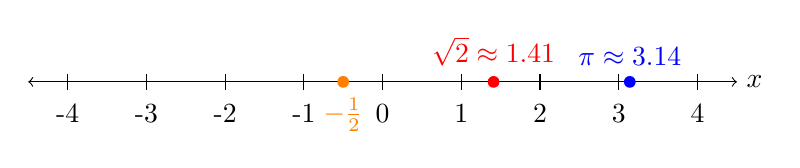
\begin{tikzpicture}[scale=1.0]
        \draw[<->] (-4.5,0) -- (4.5,0) node[right] {$x$};
        \foreach \x in {-4,-3,-2,-1,0,1,2,3,4} {
            \draw (\x, -0.1) -- (\x, 0.1);
            \node at (\x, -0.4) {\x};
        }
        \node[blue, circle, fill, inner sep=1.5pt, label=above:{\color{blue}$\pi \approx 3.14$}] at (3.14, 0) {};
        \node[red, circle, fill, inner sep=1.5pt, label=above:{\color{red}$\sqrt{2} \approx 1.41$}] at (1.41, 0) {};
        \node[orange, circle, fill, inner sep=1.5pt, label=below:{\color{orange}$-\frac{1}{2}$}] at (-0.5, 0) {};
    \end{tikzpicture}
    \caption{បន្ទាត់ចំនួនពិតបង្ហាញពីទីតាំងនៃចំនួនគត់, សនិទាន, និងអសនិទាន។}
\end{figure}

\section{ប្រមាណវិធីលើចំនួនពិត}
\subsection{ការបូក និងដក}
ការបូកនិងដកចំនួនពិតអនុវត្តតាមវិធានដូចគ្នានឹងចំនួនគត់ដែរ ទាក់ទងនឹងសញ្ញា។
\begin{itemize}[label=-]
    \item \textbf{បូកឬដកចំនួនសនិទាន៖} ប្រើភាគបែងរួមសម្រាប់ប្រភាគ ឬតម្រឹមខ្ទង់ទសភាគ។\\
    ឧទាហរណ៍៖ $2.5 + 0.75 = 3.25$
    \item \textbf{បូកឬដកចំនួនអសនិទាន៖} អាចបូកឬដករ៉ាឌីកាល់ដូចគ្នាបាន។\\
    ឧទាហរណ៍៖ $5\sqrt{2} + 3\sqrt{2} = (5+3)\sqrt{2} = 8\sqrt{2}$។ ប៉ុន្តែ $4\sqrt{3} + 2\sqrt{5}$ មិនអាចបង្រួមបានទេ។
\end{itemize}

\subsection{ការគុណ និងចែក}
\begin{itemize}[label=-]
    \item \textbf{សញ្ញាដូចគ្នា៖} ផលគុណ ឬផលចែកជាចំនួនវិជ្ជមាន។\\
    ឧទាហរណ៍៖ $(-2.5) \times (-4) = 10$
    \item \textbf{សញ្ញាផ្ទុយគ្នា៖} ផលគុណ ឬផលចែកជាចំនួនអវិជ្ជមាន។\\
    ឧទាហរណ៍៖ $15 \div (-3) = -5$
    \item \textbf{គុណឬចែករ៉ាឌីកាល់៖} $\sqrt{a} \times \sqrt{b} = \sqrt{ab}$ និង $\frac{\sqrt{a}}{\sqrt{b}} = \sqrt{\frac{a}{b}}$ (សម្រាប់ $a \ge 0, b > 0$)។\\
    ឧទាហរណ៍៖ $\sqrt{3} \times \sqrt{12} = \sqrt{36} = 6$
\end{itemize}

\section{ឧទាហរណ៍អនុវត្ត}
\begin{example}{ការចំណាត់ថ្នាក់ចំនួន}
    ចាត់ថ្នាក់ចំនួនខាងក្រោមជាចំនួនសនិទាន ឬអសនិទាន៖ $-7, \frac{9}{2}, \sqrt{25}, \sqrt{10}$។
    \begin{solution}
        \begin{itemize}
            \item $-7 = \frac{-7}{1}$ ជាចំនួនសនិទាន។
            \item $\frac{9}{2}$ ជាចំនួនសនិទាន។
            \item $\sqrt{25} = 5 = \frac{5}{1}$ ជាចំនួនសនិទាន។
            \item $\sqrt{10} \approx 3.1622...$ ជាចំនួនអសនិទាន (ទសភាគមិនចេះចប់ មិនមានខួប)។
        \end{itemize}
    \end{solution}
\end{example}

\begin{example}{ការគណនាជាមួយចំនួនពិត}
    គណនា៖ $(3\sqrt{5}) \times (2\sqrt{5}) - 10$។
    \begin{solution}
        $(3\sqrt{5}) \times (2\sqrt{5}) - 10 = (3 \times 2) \times (\sqrt{5} \times \sqrt{5}) - 10 = 6 \times 5 - 10 = 30 - 10 = 20$។
    \end{solution}
\end{example}

\section{លំហាត់អនុវត្ត}
\begin{enumerate}[label=\arabic*.]
    \item ចាត់ថ្នាក់ចំនួននីមួយៗជាសនិទាន ឬអសនិទាន៖ $0, -4.5, \sqrt{81}, \sqrt{7}, \frac{\pi}{2}$។
    \item ប្រៀបធៀបដោយប្រើ $<, >,$ ឬ $=$៖ $\sqrt{9} \_\_ 3$។
    \item ប្រៀបធៀបដោយប្រើ $<, >,$ ឬ $=$៖ $3.14 \_\_ \pi$។
    \item គណនា៖ $7\sqrt{3} - 2\sqrt{3}$។
    \item គណនា៖ $\frac{5}{2} + 1.5$។
    \item គណនា៖ $\sqrt{8} \times \sqrt{2}$។
    \item គណនា៖ $(-4.2) \div 2$។
\end{enumerate}

\section{ចម្លើយលំហាត់អនុវត្ត}
\begin{enumerate}[label=\arabic*.]
    \item សនិទាន ($0, -4.5, \sqrt{81}=9$), អសនិទាន ($\sqrt{7}, \frac{\pi}{2}$)។
    \item $\sqrt{9} = 3$។
    \item $3.14 < \pi$ (ព្រោះ $\pi \approx 3.14159...$)។
    \item $7\sqrt{3} - 2\sqrt{3} = 5\sqrt{3}$។
    \item $\frac{5}{2} + 1.5 = 2.5 + 1.5 = 4$។
    \item $\sqrt{8} \times \sqrt{2} = \sqrt{16} = 4$។
    \item $(-4.2) \div 2 = -2.1$។
\end{enumerate}
